% http://en.wikibooks.org/wiki/LaTeX/Title_Creation
% Adjusted for EPFL template


\begin{titlepage}

\begin{center}

\raisebox{2cm}[-2cm][-2cm]{
\hspace{-1.5cm}

  \footnotesize
  \begin{tabular}{@{\hspace{0pt}}l@{\hspace{0pt}} l@{\hspace{10pt}}}
    \cline{1-1}     & \multirow{5}{*}{\hspace{10pt}\raisebox{-1ex}{
\includegraphics[width=0.4\columnwidth]{EPFL_LOG_QUADRI_Red}}}\\
    EIDGEN\"{O}SSISCHE TECHNISCHE HOCHSCHULE LAUSANNE \\
    POLITECNICO FEDERALE DI LOSANNA  \\
    SWISS FEDERAL INSTITUTE OF TECHNOLOGY LAUSANNE  \\
    \cline{1-1} \\
    \raisebox{0.5ex}{\textbf{School of Computer and Communication Sciences}} \\
    \raisebox{1.2ex}{Computer Science Section | Distributed Systems Laboratory (LSIR)} \\
    %\scriptsize CH -- 1015 LAUSANNE \\

  \end{tabular}%
}

\vspace{1\baselineskip}
\Huge

\newcommand{\HRule}{\rule{\linewidth}{0.3mm}}


    {\huge \bfseries  CERN Digital Library  } \\
    {\Large \bfseries  MASE(CDS): A Math Aware Search Engine (for CDS)} \\
	\vspace{3mm}    
    \textsc{\Large Master Thesis Project} \\
    
    %\HRule \\[0.2cm]
	
	\vspace{3mm}
	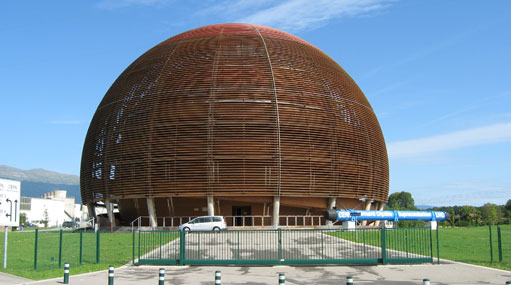
\includegraphics[height=6 cm]{cern_logo1.jpg}
	\vspace{3mm}
	\HRule 
	
	\emph{Autor:} \\
	Arthur \textsc{Oviedo}\\
    \vspace{0.5cm}
    \emph{Supervisors:} \\   

    CERN: Nikolaos \textsc{Kasioumis} \\   
    EPFL: Karl \textsc{Aberer}\\

	\vspace{0.5cm}
    % Bottom of the page
    %\emph{Remis le: 8 janvier 2010}
	%{\large \today}


\end{center}


\end{titlepage}

\newpage
\thispagestyle{empty}
\mbox{}